\documentclass[conference]{IEEEtran}
\IEEEoverridecommandlockouts
% The preceding line is only needed to identify funding in the first footnote. If that is unneeded, please comment it out.
\usepackage{cite}
\usepackage{amsmath,amssymb,amsfonts}
\usepackage{algorithmic}
\usepackage{textcomp}
\usepackage{xcolor}
\usepackage{colortbl}
\usepackage[rightcaption]{sidecap}
\usepackage{wrapfig}
\usepackage{adjustbox}
\usepackage{siunitx}
\usepackage{hyperref}
\def\UrlBreaks{\do\/\do-}
\usepackage{graphicx} %package to manage images
\graphicspath{ {./images/} }


\def\BibTeX{{\rm B\kern-.05em{\sc i\kern-.025em b}\kern-.08em
    T\kern-.1667em\lower.7ex\hbox{E}\kern-.125emX}}
\begin{document}

\title{Online Store Application: Art Store+}

\author{\IEEEauthorblockN{1\textsuperscript{st} Tomás Marcos}
\IEEEauthorblockA{\textit{Faculdade de Ciências Exatas e da Engenharia} \\
\textit{Universidade da Madeira}\\
Funchal, Portugal \\
2037017@student.uma.pt}
\and
\IEEEauthorblockN{2\textsuperscript{nd} Nelson Vieira}
\IEEEauthorblockA{\textit{Faculdade de Ciências Exatas e da Engenharia} \\
\textit{Universidade da Madeira}\\
Funchal, Portugal \\
2080511@student.uma.pt}
\and
\IEEEauthorblockN{3\textsuperscript{rd} Luís Olim}
\IEEEauthorblockA{\textit{Faculdade de Ciências Exatas e da Engenharia} \\
\textit{Universidade da Madeira}\\
Funchal, Portugal \\
2034717@student.uma.pt}
}

\maketitle

\begin{abstract}
 \\Utilizar arte para decorar espaços, tanto privados, como uma casa, ou público não é algo novo. Existem vários leilões para compra de arte, mas estes normalmente não são acessíveis a todos devido aos preços elevados das obras nestes e também dificuldade de sequer encontrá-los. Isto normalmente leva a que a melhor opção para compra de arte seja em lojas de decoração, mas esta arte costuma ser algo produzido em massa. Neste artigo iremos falar de uma aplicação que pretende resolver estes problemas, oferecendo uma loja fácil de aceder onde pessoas do público geral possam comprar artigos de arte a preços acessíveis, mas também uma plataforma que permita a artistas locais e pouco conhecidos a arrancarem a sua carreira e criarem um nome para si mesmos.
\end{abstract}

\begin{IEEEkeywords}

\end{IEEEkeywords}

\section{Introdução}

\IEEEPARstart{A}rte, do latin ars que significa técnica e/ou habilidade, pode ser entendida 
como a atividade humana ligada às manifestações de ordem estética ou comunicativa, realizada 
por meio de uma grande variedade de linguagens, tais como: arquitetura, desenho, escultura, 
pintura, escrita, música, dança, teatro e cinema, em suas variadas combinações. \cite{wikiarte}

`Desde sempre a arte funcionou como espelho da sociedade, 
acompanhando cada contemporaneidade ao longo dos tempos, deixando registado na sua obra os diferentes 
momentos vividos, com intensidade e questionamento, como um diário pessoal da humanidade, 
desde que o Homem se pensou como tal.` \cite{patrimonio}

Como referido, arte pode ter várias formas e é bastante comum uma pessoa decorar a sua casa com objetos artísticos, como quadros ou estátuas. Normalmente este tipo de arte é encontrado em lojas mas são apenas itens produzidos em massa. Isto cria um problema para quem gosta de ter algo único. Não é fácil encontrar um lugar para arranjar artigos únicos atualmente. Maior parte desta arte é vendida por leilões, mas estes leilões costumam vender arte de artistas já conhecidos, o que leva a preços bastante elevados, algo que maior parte das pessoas não consegue comprar. Isto em si também torna difícil de novos talentos emergirem e exporem a sua arte, sendo que maior parte dos artistas novos/menos conehcidos vendem a sua arte em feiras ou pelas redes sociais ou então acabam por doar para exposições, nunca recebendo exposição merecida.

É com isto que decidimos criar esta aplicação, Art Store+. Com esta aplicação pretendemos criar uma loja online onde artistas podem expor as suas criações e começar uma carreira e também pessoas do público geral podem procurar e comprar arte para decoração ou coleção a preços acessíveis.


\subsection{Formas de arte}
As artes são, muitas vezes, divididas em categorias específicas, tais como artes decorativas, 
artes plásticas ou visuais, artes do espectáculo, ou literatura.

\subsection{Objetivos}
\begin{itemize}
    \item Tornar obras de arte mais acessíveis ao público geral;
    \item Reconhecimento a artistas menos conhecidos;
    \item Fazer com que artistas novos surgir no mercado;
    \item Promover talento local;
\end{itemize}

\section{Métodos e Metadologias}

O trabalho descrito neste artigo pretende 

\subsection{Tecnologias utilizadas}

A aplicação que propomos, é uma aplicação que foi desenvolvida utilizando:

\begin{itemize}
    \item Figma - software de prototipagem;
    \item FlutterFlow - aplicação web para desenvolvimento de aplicações à base de Flutter;
    \item Flutter - linguagem para desenvolvimento de aplicações móveis;
    \item Firebase - plataforma para desenvolvimento de aplicações, atualmente pertencente à Google;
    \item Firestore - base de dados do Firebase;
    \item VSCode - IDE utilizado para escrita do código;
    \item Git - plataforma de controlo de versões;
\end{itemize}

Primeiramente, foram realizados alguns esboços sobre qual poderia ser a aparência da aplicação. A figura \ref{fig:sketches} 
mostra os esboços realizados para a aplicação.

\begin{figure}[ht]
    \centering
    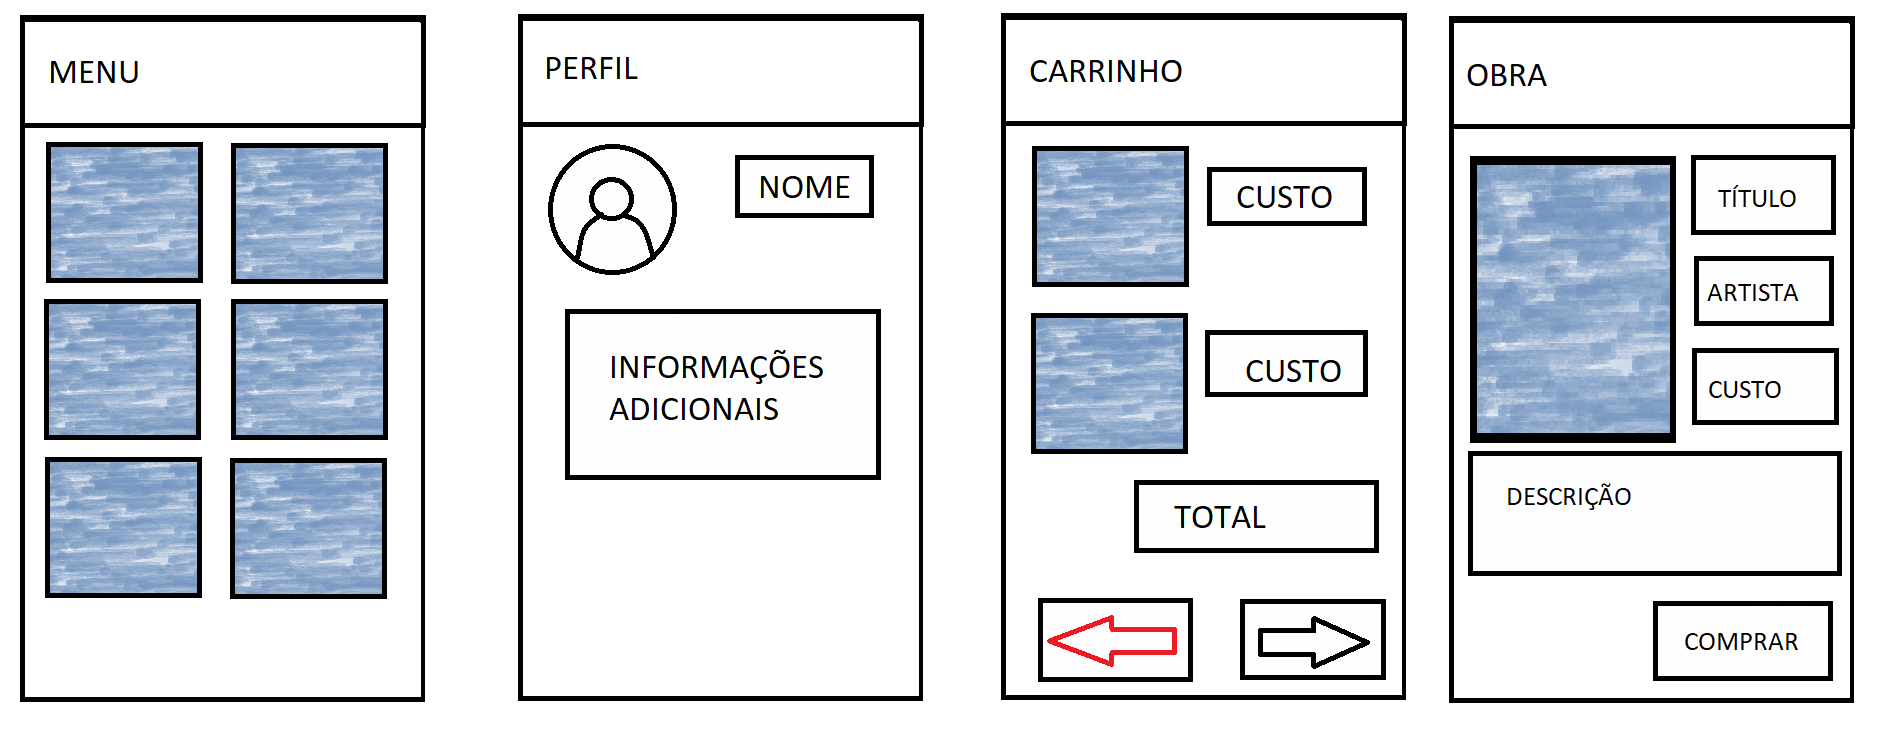
\includegraphics[width=0.5\textwidth]{appsketches.png}
    \caption{Esboços da aplicação}
    \label{fig:sketches}
\end{figure}

Desenhou-se um esquema representativo da navegação na aplicação, como mostra a figura \ref{fig:navmap}

\begin{figure}[ht]
    \centering
    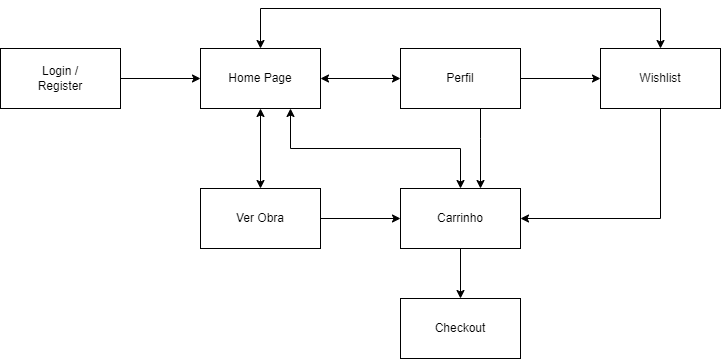
\includegraphics[width=0.5\textwidth]{artstore+map.drawio.png}
    \caption{Mapa de Navigação}
    \label{fig:navmap}
\end{figure}

Como se pode observar, pelo mapa, o utilizador ao iniciar a aplicação será capaz de realizar Login ou Registo. 
Após feito o Login, o utilizador será redirecionado para a Home Page. A partir da Home Page, o utilizador poderá 
navegar para outras páginas, tais como verificar o seu perfil, verificar o carrinho e a sua Wishlist. Também, 
será na Home Page que serão expostas as obras de arte, nos quais o utilizador poderá visitar a página de cada obra. 

O utilizador poderá concluir a compra das obras na página de Checkout, que pode ser acedida pelo Carrinho.

A partir dos esboços criados, procedeu-se à realização de um protótipo no Figma, de maior fidelidade, tal que 
fosse possível testar algumas funcionalidades da aplicação.

\subsection{Testes}

Relativamente aos testes da aplicação, testámos utilizando uma versão de produção da app. Realizámos os testes com sete utilizadores e depois dos testes foi pedido a estes que realizassem um questionário relativamente à usabilidade da aplicação. Dois dos sete utilizadores não quiseram responder ao questionário, porque não queriam o seu nome em nenhum registo apesar de explicarmos que não iríamos guardar informação sobre estes. Apesar disto tirámos proveito dos testes de cada utilizador através do método think aloud. Demos um conjunto de tarefas para os utilizadores realizarem, sendo estas:

\begin{itemize}
    \item Registar e fazer login;
    \item Localizar uma certa obra(diferente para cada utilizador) na página principal e comprar essa peça;
    \item Verificar o perfil e editar o perfil;
    \item Verificar o carrinho de compras;
\end{itemize}

Estes testes tinham como objetivo principal avaliar a usabilidade e navegação da aplicação. Relativamente a estes obtivemos resultados maioritariamente positivos. Os utilizadores acharam todos que a app era fácil de navegar e também gostaram da maneira que a informação sobre as peças de arte era disponibilizada. A figura
\ref{fig:navegacaoTest}
mostra os resultados do questionário relativamente à facilidade dos utilizadores a navegar na aplicação e a figura
\ref{fig:facilitaTest}
mostra os resultados relativamente a se os utilizadores acham que esta aplicação facilitaria o processo de compra de arte.

\begin{figure}[ht]
    \centering
    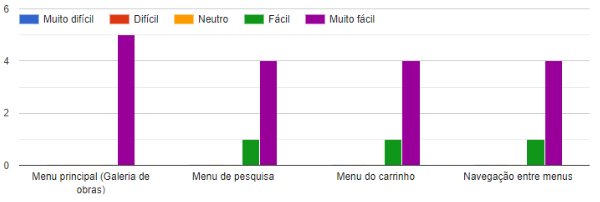
\includegraphics[width=0.5\textwidth]{questionarioNavegacao.png}
    \caption{Resultados do questionário para a navegação na app}
    \label{fig:navegacaoTest}
\end{figure}

\begin{figure}[ht]
    \centering
    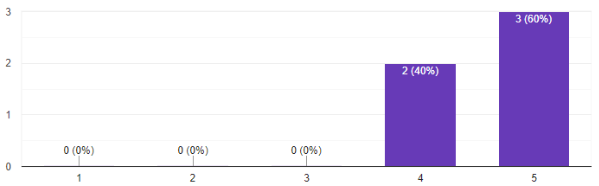
\includegraphics[width=0.5\textwidth]{questionarioFacilitar.png}
    \caption{Resultados do questionário para a navegação na app}
    \label{fig:facilitaTest}
\end{figure}

Como podemos ver pelos resultados, os utilizadores tiverem muita facilidade a navegar pela a aplicação e acharam que esta aplicação iria de facto facilitar o processo de compra de arte.

O ponto mais negativo mencionado pelos utilizadores foi a falta de opções de filtragem/procura. Para a versão utilizada para testes ainda não tínhamos implementado estas funcionalidades, mas já era algo planeado implementar na aplicação.

Outra observação foi o facto de na página principal não mostrar os preços das obras antes de irmos para a página da obra. Não tínhamos pensado nisto inicialmente, mas é algo que faz sentido, pois lojas online normalmente têm o preço do item a ser mostrado sem que a pessoa tenha que clicar neste e abrir outra página. Isto foi implementado depois dos testes.

\subsection{Problemas Encontrados}

Durante a realização do projeto descrito neste artigo, surgiram vários problemas, 

\section{Conclusão e Trabalho Futuro}

Neste trabalho conseguimos criar uma aplicação que cumpre os nossos objetivos. Também conseguimos através dos testes realmente ver que as pessoas não têm muita facilidade a encontrar lugares para comprar arte, sendo que maior parte deles não sabiam de nenhum lugar para comprar e os que sabiam mencionaram que estes lugares não eram fáceis de encontrar.

Trabalho futuro para este projeto inclui trabalho na base de dados, implementar filtros/pesquisa para as obras de arte, o planeado sendo através de tags para o tipo de arte e também pesquisa pelo artista em si, adicionar mais peças de arte, para o protótipo utilizámos peças conhecidas que nunca iriam estar no produto final, simplesmente utilizámos estas pois são reconhecíveis e assim os utilizadores dos testes iriam entender imediatamente o objetivo da app e por fim implementar/melhorar páginas de artistas.

Concluindo, conseguimos desenvolver um protótipo com as funcionalidades principais da aplicação e que mostra o que esta irá fazer. A partir dos testes também conseguimos perceber melhor o que a app deve de fazer e mostrar ao utilizador e também, a partir dos testes, vimos que estamos no caminho certo no desenvolvimento desta aplicação.

\bibliographystyle{IEEEtran}
\bibliography{references}

\end{document}


